\documentclass[11pt]{article}

%	packages
\usepackage{tikz}
\usepackage{authblk}
\usepackage{amsmath}
\usepackage{amssymb} 
\usepackage{caption}
\usepackage{graphicx}
\usepackage[hypertexnames=false,colorlinks=true,linkcolor=blue,citecolor=blue]{hyperref}
\usepackage[numbers,comma,square,sort&compress]{natbib}
\usepackage[a4paper,text={6.5in,10in},centering]{geometry}
\usepackage{subcaption}
%	code syntax higlighting
\usepackage{listings}
\usepackage{color}
\usepackage{textcomp}
\definecolor{listinggray}{gray}{0.9}
\definecolor{lbcolor}{rgb}{0.9,0.9,0.9}
% C++ = [Visual]C++ ; matlab = matlab
\lstset{
	backgroundcolor=\color{lbcolor},
	tabsize=4,
	rulecolor=,
	language=java,
	keywordstyle=\bfseries\ttfamily\color[rgb]{0,0,1},
	identifierstyle=\ttfamily,
	commentstyle=\color[rgb]{0.133,0.545,0.133},
	stringstyle=\ttfamily\color[rgb]{0.627,0.126,0.941},
	showstringspaces=false,
	basicstyle=\small,
	%numberstyle=\footnotesize,
	%numbers=left,
	stepnumber=1,
	numbersep=10pt,
	tabsize=2,
	breaklines=true,
	prebreak = \raisebox{0ex}[0ex][0ex]{\ensuremath{\hookleftarrow}},
	breakatwhitespace=false,
	aboveskip={1.5\baselineskip},
  columns=fixed,
  upquote=true,
  extendedchars=true,
 frame=single,
% backgroundcolor=\color{lbcolor},
}


%	figures
\graphicspath{{eps/}{pdf/}{../figs//}}
%\setcaptionmargin{0.25in}
\def\captionfont{\itshape\small}
\def\captionlabelfont{\upshape\small}

%	counters
\makeatletter\@addtoreset{equation}{section}\makeatother
\renewcommand{\theequation}{\arabic{section}.\arabic{equation}}


%%%%%%%%%%%%%%%%%%%%%%%%%%%%%%%%%%%%%%%%%%%%%%%%%%%%%%%%%%%%%%%%%%%%%%%%%%%%

\begin{document}

\title{Equation-free analysis of agent-based models:\\Stochastic Double Potential Well}

%\author[1]{Spencer A. Thomas}
\author{Spencer A. Thomas}
\author{David J.B. Lloyd}
\author{Anne C. Skeldon}
%\affil[1]{\small Department of Mathematics, Evolution and Resilience of Industrial Ecosystems (ERIE), University of Surrey, Guildford, GU2 7XH, UK}
\affil{\small Department of Mathematics, Evolution and Resilience of Industrial Ecosystems (ERIE), University of Surrey, Guildford, GU2 7XH, UK}
\date{\today}
\maketitle


%%%%%%%%%%%%%%%%%%%%%%%%%%%%%%%%%%%%%%%%%%%%%
% stochastic double well
%%%%%%%%%%%%%%%%%%%%%%%%%%%%%%%%%%%%%%%%%%%%%

\section{The Model: An Overview}

Consider a system with a hill between two valleys as in Fig.~\ref{fig:DDW}. A ball will tend to roll down into one of the valleys where it will remain at rest (filled circles in Fig.~\ref{DWP}). The system is in equilibrium when the ball is at rest, and the state of the system (here position of the ball) at an equilibrium is known as a fixed point. Which of these valleys the ball will roll into to depends on the initial conditions of the system, i.e. which side of the hill it starts. The ball may also remain at rest if it is exactly at the top of the hill as shown in Fig.~\ref{DWP} as an empty circle. For the filled circles, if one moves the ball slight to the left or right it will roll back down to the bottom of the valley where it started. This is known as a stable fixed point as small changes to the state of the system will result in the same outcome, rolling to the bottom of the valley. The top of the hill, however, is known as an unstable fixed point, as any slight change to the position of the ball will cause it to roll down the hill and into one of the valleys. The valley the ball ends up in depends on the direction of the change to the system, i.e. which way you move the ball. If we reduce the height of the hill the position of these fixed points change, and to a point the behaviour remains the same, see Fig.~\ref{fig:DDW}. It is clear from Fig.~\ref{fig:DDW} that there is a dependence of the location of these fixed points and the height of the hill. If we reduce the hill height even more, what happens? What if we add noise to the system, so the ball is constantly moving, or that the exact location of the fixed points varies between simulations of the system? How does this effect the unstable point which is sensitive to change?


\begin{figure}[t]
	\centering
	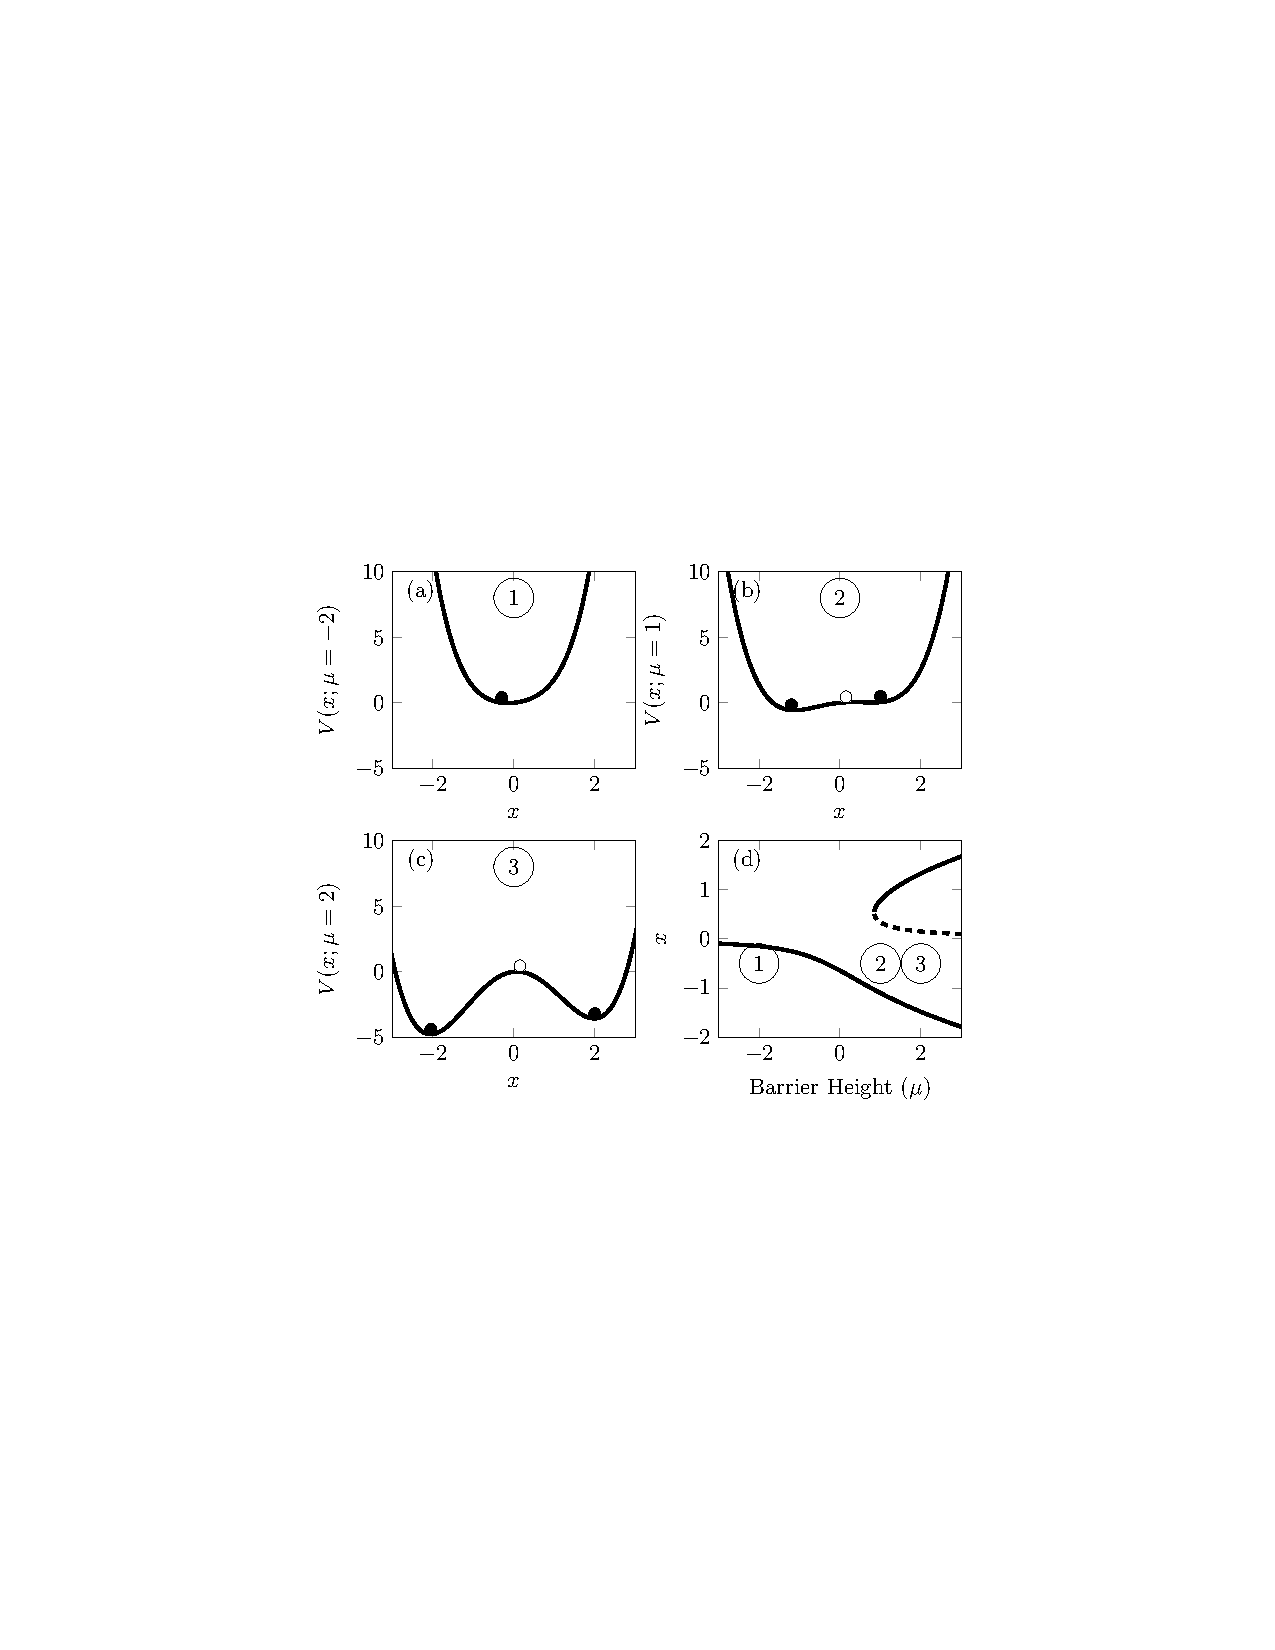
\includegraphics[width=0.75\linewidth, trim=5cm 9cm 5cm 9cm, clip=true]{DoubleWell}
	\caption{Double well potential for differing values of barrier height ($\mu$) as indicated on the $y$-label and bifurcation curve for the system. Stable (unstable) states are indicated by black (white) circles and solid (dashed) lines. \label{fig:DDW}}
\end{figure}

\section{The Model: Details} 
\label{sec:details}
The stochastic double well is modelled with a potential;
\begin{equation}
	\frac{dV(x)}{dx} = -x(x^2 - \mu) - \nu~,
\end{equation}
	where $\mu$ is the barrier hight and $\nu$ is the asymmetric term in the well. The state of a particle in the well is given by;
\begin{equation}
	\dot{x} = \frac{dV(x)}{dx} + \eta\dot{W}~,
\end{equation}
	where $\eta$ is the noise level and $\dot{W}$ is Gaussian noise between 0 and 1. Though not an ABM, this is coded in NetLogo with our algorithm `wrapped around' it to compute the fixed points of the system determined through our equation-free continuation. In this analysis we set $\eta=\sqrt{dt}$, where $dt$ is the step size in the ODE solver.


\section{Requirements of the User}
The user defined settings in the input file are given below. 
\begin{lstlisting}
String NetlogoFile = "netlogo/doubleWell.nlogo"; 
String[] systemParameters = {"set barrier-height", "set asymmetry-term"}; 
double[] param = {3.5, 0.3};  
String[] Measure	= {"x"};
String[] LiftOperator = {"set x"}; 
double[] Initial	= {0.0}; 
boolean isSystemInitialised = true;  
\end{lstlisting}		
	Here the {\tt NetlogoFile} is a string of text with the location of the NetLogo file, here contained in the sub-folder {\it netlogo}. {\tt Lift} is the name of the parameters required to set up with system, which correspond to the values in {\tt param}. Note the parameter you wish to vary in order to analyse the system with this package goes first in this list. {\tt systemParameters} are the parameters are the parameters you wish to monitor during this analysis which take the initial value of {\tt Initial} as an estimate of the first fixed point of the system. Note there can be any number of {\tt systemParameters} in your system. {\tt Measure} is the output measure of the system, note this is not the same as {\tt systemParameters} in general.

\section{Outcome of Equation-free Analysis}

We focus on the saddle-node branch of the SDW model due to the presence of a bifurcation unlike the lower stable branch. Using the system exploration phase to determine the essential continuation parameters we obtain $N=100$, $\tau=1.0$ and $\delta s=0.05$. With these parameters we use our algorithm to perform EF continuation of the SDW NetLogo code following the equilibria around the fold as indicated in Fig.~\ref{fig:SDW}. Note the successful continuation past the bifurcation point despite the large value of $\tau$ and small number of realisations $N$ compared to other EF continuation of SDW \cite{Barkley2006}, where $\tau=0.1$ and $N=10^4$ in the majority of the simulations. Our algorithm is successful in continuation of the SDW at large time horizons and a low number of realisation simultaneously, in addition to systematically determining the problem specific parameters prior to the continuation process. Interestingly we note that the variance of this system is the same along both the stable and unstable branches, and, moreover, near the fold. This indicates that the variance of the system is not dependent on the stability of the branch and is due to the noise in the system, which is determined by the value of $\tau$ through the $\eta\dot{W}$ term in Eq.~(\ref{eq:SDW}. 


\begin{figure}[t]
	\centering
	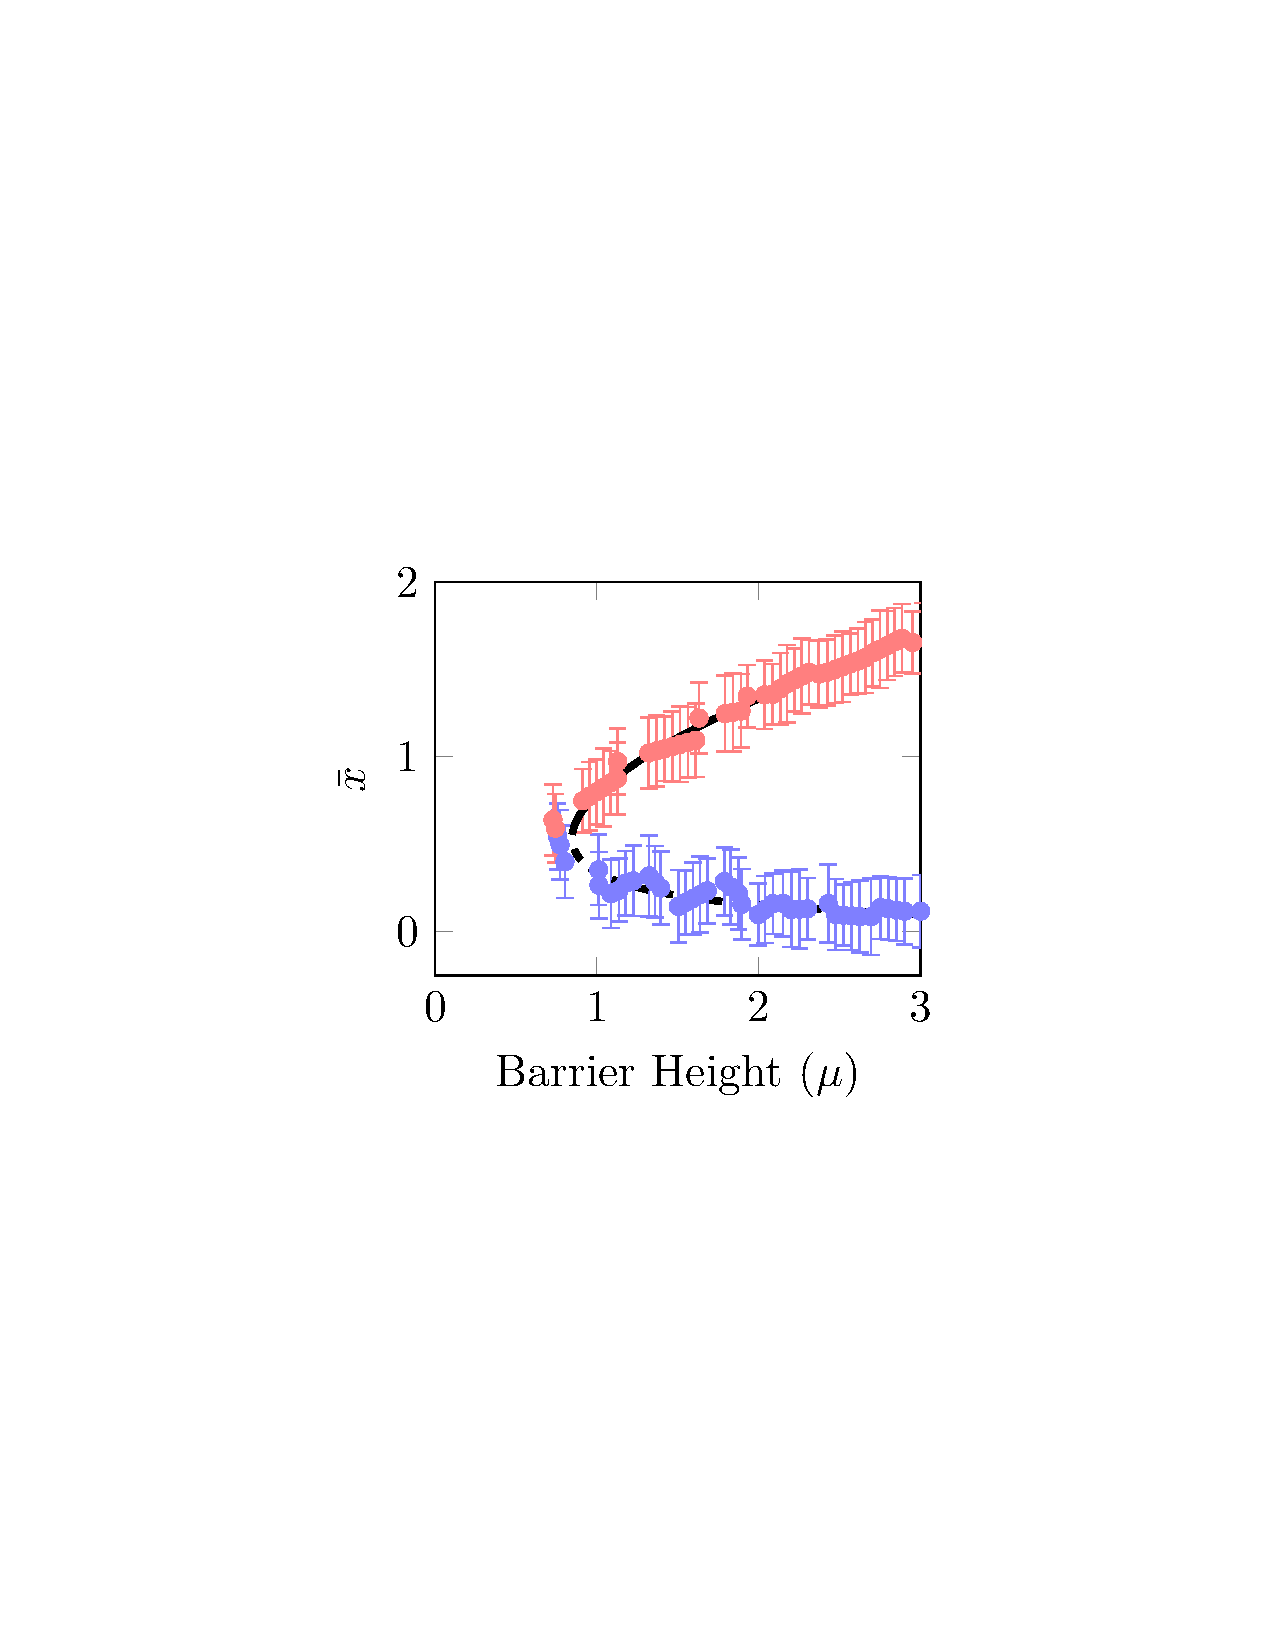
\includegraphics[width=0.5\linewidth, trim=5cm 9cm 5cm 9cm, clip=true]{StochasticDoubleWell}	
	\caption{Continuation of a stochastic double well potential is compared to the deterministic case (right) with where stable (unstable) branches are illustrated by red (blue) points. Error bars are $\pm$ two standard errors, $\tau$ = 1.0, $N$ = 100 and $\delta s$ = 0.05. \label{fig:SDW}}
\end{figure}
 
\section{Further Reading}

The following table contains a reference list for further reading on the topic contained in this method and example. 
\begin{center}
\begin{tabular}{|l|c|}
\hline
Topic									&	Reference \\ \hline
Introduction to bifurcation analysis		&	\cite{Meunier1988}	\\
Introduction to continuation 			&	\cite{Doedel1991,Allgower1990,Rheinboldt2000,Krauskopf2007} \\ 
Introduction to equation-free methods	&	\cite{Theodoropoulos2000,Kevrekidis2003,Kevrekidis2009}	\\
Double well potential 					&	\cite{Mahato1998,Zhu2013,Ditlevsen2010}	\\
Continuation of double well potential	&	\cite{Barkley2006,Kuehn2013}	\\
\hline
\end{tabular}
\end{center}



\section*{Acknowledgments}
{The support of the UK Engineering and Physical Sciences Research Council for programme grant EP/H021779/1 (Evolution and Resilience of Industrial Ecosystems (ERIE)) is gratefully acknowledged.}
 
 
\begin{thebibliography}{10}  

\bibitem{Meunier1988}
{\sc C. Meunier and A. D. Verga},
{\it Noise and Bifurcations}
J. Stat. Phys., 1988, 50(1-2), pp 345-375

\bibitem{Doedel1991}
{\sc E. Doedel, H. B. Keller and J. P. Kernevez},
{\it Numerical Analysis And Control of Bifurcation Problems (I) Bifurcation in Finite Dimensions}
Int. J. Bifurcation Chaos, 1991, 493(3), pp 493-520

\bibitem{Allgower1990}
{\sc E. L. Allgower and K. Georg},
{\it Numerical Continuation Methods, An Introduction}
Springer-Verlag Berlin Heidelberg 1990

\bibitem{Rheinboldt2000}
{\sc W. C. Rheinboldt},
{\it Numerical continuation methods: a perspective}
Journal of Computational and Applied Mathematics, 200, 124, pp 229-244

\bibitem{Krauskopf2007}
{\sc B. Krauskopf, H. M. Osinga and J. Gal\`{a}n-Vioque (Eds.)},
{\it Numerical Continuation Methods for Dynamical Systems}
Springer 2007

\bibitem{Theodoropoulos2000}
{\sc C. Theodoropoulos, Y. H. Qian and I. G. Kevrekidis IG}
{\it Coarse stability and bifurcation analysis using time-steppers: a reaction-diffusion example}
Proc. Natl. Acad. Sci. 2000, 97, pp 9840-9845

\bibitem{Kevrekidis2003}
{\sc I. G. Kevrekidis et al.} 
{\it Equation-free, coarse-grained multiscale computation: enabling microscopic simulators to perform system-level tasks}
Comm. Math. Sci. 2003, 1, pp 715-762 

\bibitem{Kevrekidis2009}
{\sc I. G. Kevrekidis and G. Samaey},
{\it Equation-Free Multiscale Computation: Algorithms and Applications},
Annual Review of Physical Chemistry, 2009, 60(1), pp 321-344

\bibitem{Mahato1998}
{\sc M. C. Mahato and A. M. Jaynnavar},
{\it Some stochastic phenomena in a driven double-well system},
Physica A, 1988, 248, pp 138-154

\bibitem{Zhu2013}
{\sc W. Q. Zhu, G. Q. Cai and R. C. Hu},
{\it Stochastic analysis of dynamical system with double-well potential},
Int. J. Dynam. Control, 2013, 1, pp 12-19

\bibitem{Ditlevsen2010}
{\sc P. D. Ditlevsen and S. J. Johnsen},
{\it Tipping points: Early warning and wishful thinking},
GEOPHYSICAL RESEARCH LETTERS, 2006, 37(L19703), pp 1-4

\bibitem{Barkley2006}
{\sc D. Barkely, I. G. Keverekidis and A. M. Stuart},
{\it The Moment Map: Nonlinear Dynamics of Density Evolution via a Few Moments},
SIAM J. Applied Dynamical Systems, 2006, 5(3), pp 403-434

\bibitem{Kuehn2013}
{\sc C. Kuehn},
{\it Deterministic continuation of stochastic metastable equilibria via Lyapunov equations and ellipsoids}
ArXiv e-prints, 2013, 1106.3479, pp 1-29




\end{thebibliography} 

\end{document} 

